% =============================================================================
%  NEUROGUARD: Zero-Day IoT Compromise Detection via Siamese Behavioral
%  Fingerprinting
%
%  Target journal: IEEE Transactions on Information Forensics and Security
%  Document class: IEEEtran (journal mode, 10pt, two-column)
%  Compile: pdflatex → bibtex → pdflatex × 2
% =============================================================================

\documentclass[journal,10pt,twoside]{IEEEtran}

% ---------------------------------------------------------------------------
% Packages
% ---------------------------------------------------------------------------
\usepackage[T1]{fontenc}
\usepackage[utf8]{inputenc}
\usepackage{amsmath,amssymb,amsfonts}
\usepackage{algorithmic}
\usepackage{graphicx}
\usepackage{booktabs}        % professional table rules
\usepackage{xcolor}
\usepackage{url}
\usepackage{microtype}       % better justification
\usepackage{cite}            % IEEE-style citation compression [1]--[3]
\usepackage{dblfloatfix}     % fix float placement in two-column mode
\usepackage{multirow}

% ---------------------------------------------------------------------------
% Hyper-references (comment out for camera-ready if venue requires)
% ---------------------------------------------------------------------------
\usepackage[colorlinks=true,linkcolor=blue,citecolor=blue,urlcolor=blue]{hyperref}

% ---------------------------------------------------------------------------
% Theorem-like environments
% ---------------------------------------------------------------------------
\newtheorem{definition}{Definition}
\newtheorem{proposition}{Proposition}

% ---------------------------------------------------------------------------
% Custom commands
% ---------------------------------------------------------------------------
\newcommand{\neuroguard}{\textsc{NeuroGuard}}
\newcommand{\norm}[1]{\left\lVert #1 \right\rVert}
\newcommand{\R}{\mathbb{R}}

% =============================================================================
\begin{document}

\title{\neuroguard: Zero-Day IoT Compromise Detection\\
       via Siamese Behavioral Fingerprinting}

\author{Sagar~Bhetuwal%
  \thanks{S. Bhetuwal is with the Department of Computer Science.
          E-mail: \texttt{sagarbhetuwal@example.edu}.}
\IEEEmembership{}
}

\markboth{IEEE Transactions on Information Forensics and Security,~Vol.~XX,
          No.~XX,~2026}%
         {\neuroguard{}: Zero-Day IoT Compromise Detection via Siamese
          Behavioral Fingerprinting}

\maketitle

% =============================================================================
\begin{abstract}
Existing intrusion detection systems for IoT networks rely on known attack
signatures, making them blind to threats they have never seen.
We present \neuroguard{}, a zero-day IoT compromise detection system that
learns what normal behavior looks like for each individual device and raises
an alert when a device stops acting like itself --- without ever training on
attack data.

The system uses a Siamese neural network to map 50-flow traffic windows
into a 64-dimensional behavioral embedding space. A shared encoder
combining feedforward layers with a Transformer self-attention block
is trained with contrastive loss on pairs of normal windows, so that windows
from the same device cluster together while windows from different devices
are pushed apart. Each device is then enrolled by computing a baseline
centroid from held-out normal traffic; a new window triggers an alert if its
embedding is too far from that centroid.

Evaluated on the TON\_IoT dataset~\cite{alsaedi2020toniot} under a
strict protocol where no attack data was seen at any stage, \neuroguard{}
achieves a ROC-AUC of 0.9402, a detection rate of 97.6--98.3\%, and
an F1 score of 0.9814 across 839 attack windows spanning eight attack types.
We also introduce a lightweight EWMA-based drift detector that catches
slow, APT-style compromise that stays below the per-window alert threshold,
firing within 15--25 windows of sustained behavioral elevation.
\end{abstract}

\begin{IEEEkeywords}
IoT security, intrusion detection, zero-day threats, Siamese neural networks,
contrastive learning, behavioral fingerprinting, EWMA drift detection,
anomaly detection.
\end{IEEEkeywords}

% =============================================================================
\section{Introduction}
\label{sec:intro}

IoT devices are now embedded in nearly every part of modern life --- smart
home appliances, industrial sensors, healthcare monitors, and critical
infrastructure all rely on networked devices that are often resource-constrained
and poorly secured.
With an estimated 17 billion such devices connected worldwide~\cite{statista2023iot},
the scale of the attack surface is significant.
When one of these devices is compromised, the attacker gains a persistent
foothold in the network, often going undetected for weeks.

The core problem with defending these devices is that most intrusion detection
systems (IDS) work by comparing network traffic against a library of known
attack signatures.
This works well for attacks that have already been documented, but it completely
fails for new ones.
When the Mirai botnet spread in 2016, it compromised hundreds of thousands of
IoT devices before any signature for it
existed~\cite{antonakakis2017mirai}.
More sophisticated attackers, often called Advanced Persistent Threats (APTs),
deliberately move slowly and carefully --- staying under detection thresholds
for months before launching their final payload.
No amount of fine-tuning a signature-based IDS fixes this, because the problem
is not the parameters, it is the approach.

The observation that motivated this work is straightforward.
An IoT device with a fixed function --- a thermostat, a smart door lock, a
factory sensor --- does roughly the same things on the network every day.
It connects to the same servers, sends similar sized packets, at similar
intervals, using the same protocols.
This behavioral stability makes it possible to build a fingerprint of what that
specific device's normal traffic looks like.
Once that fingerprint exists, we no longer need to know anything about attacks.
We just need to ask: is this device still acting like itself?
If the answer is no, something is wrong.

This paper presents \neuroguard{}, a system built around that idea.
A Siamese neural network is trained on normal traffic from 16 IoT devices to
learn a behavioral embedding space where windows from the same device cluster
together and windows from different devices are well-separated.
Each device is then enrolled by computing a centroid from a small set of
held-out normal windows.
At inference time, a new traffic window is flagged as anomalous if its
embedding is too far from that device's centroid --- regardless of what kind
of attack, if any, produced it.
Because the model never trains on attack data, it has no blind spots for
unknown attack types.

The main contributions of this work are:

\begin{enumerate}
  \item \textbf{Per-device behavioral identity via contrastive learning.}
    We show that a Siamese network trained only on normal traffic can build
    per-device fingerprints that achieve an inter-to-intra class embedding
    separation ratio of $3.08\times$, sufficient for clean anomaly scoring.

  \item \textbf{Transformer-augmented behavioral encoder.}
    A Pre-LN Transformer self-attention block~\cite{xiong2020preln} within the
    shared encoder captures cross-feature behavioral correlations (e.g., the
    joint pattern of SYN ratio, ACK ratio, and connection fan-out that
    characterizes scanning), improving the separation ratio by 30\% compared
    to a feedforward-only encoder.

  \item \textbf{Enrollment-calibrated per-device thresholds.}
    Alert thresholds derived from each device's own enrollment distribution
    adapt automatically to per-device variability, requiring no manual
    threshold tuning across heterogeneous device types.

  \item \textbf{EWMA drift detection for APT-style compromise.}
    A lightweight exponentially weighted moving average detector catches
    slow, sustained behavioral drift that stays below the per-window threshold,
    firing within 15--25 windows with zero additional false positives on
    normal traffic.
\end{enumerate}

Evaluated on the TON\_IoT dataset~\cite{alsaedi2020toniot} with no attack data
used at any stage, \neuroguard{} achieves ROC-AUC 0.9402, detection rate
97.6--98.3\%, and F1\,=\,0.9814 at $k=3.0$ across 839 attack windows spanning
eight attack types.

% =============================================================================
\section{Related Work}
\label{sec:related}

\subsection{Signature-Based and Rule-Based IDS}

Tools like Snort and Suricata have been the backbone of network intrusion
detection for decades.
They match traffic against hand-written rules or known attack patterns and are
fast and interpretable.
Their limitation is that they require prior knowledge of the attack: a new
malware variant with no existing rule simply passes through.
NEUROGUARD takes the opposite approach --- it requires no knowledge of attacks
and instead focuses entirely on what normal looks like.

\subsection{ML-Based Anomaly Detection}

Unsupervised methods like IsolationForest~\cite{liu2008iforest} and
OneClassSVM~\cite{scholkopf1999ocsvm} estimate a boundary around normal
training data and flag points outside it as anomalies.
These methods do not require attack labels, which is useful.
However, when applied to multi-device IoT traffic, they pool all devices'
normal windows into one distribution, losing the per-device identity
information that makes anomaly scores meaningful.
We demonstrate this empirically in Section~\ref{sec:baselines}: both methods
achieve less than 4\% detection rate on the same data where \neuroguard{}
achieves 97.6\%.

Autoencoder-based anomaly detection --- most notably
Kitsune~\cite{mirsky2018kitsune} --- trains a network to reconstruct normal
traffic and uses reconstruction error as an anomaly signal.
Kitsune achieves strong results on single-device traces, but does not handle
the case where normal windows from multiple different device types are
present in training, which causes reconstruction quality to become
independent of device identity.

\subsection{Siamese and Contrastive Learning}

Siamese networks were originally proposed for signature
verification~\cite{hadsell2006contrastive} and have since been applied to
face recognition, speaker identification, and one-shot learning.
The key property --- that a shared encoder is trained to produce nearby
embeddings for similar inputs and distant embeddings for dissimilar ones ---
maps directly onto the per-device behavioral fingerprinting problem.
To our knowledge, this is the first application of Siamese contrastive
learning to IoT network traffic anomaly detection.

\subsection{Federated and Distributed IoT Detection}

D\"{I}oT~\cite{nguyen2019diot} uses federated learning to build device-type
behavior models without centralizing traffic data.
This addresses privacy concerns in deployment but still requires
device-type labels and does not produce per-device fingerprints.
\neuroguard{} uses per-device enrollment to achieve device-instance
specificity without requiring any attack labels or centralized infrastructure.

% =============================================================================
\section{Methodology}
\label{sec:method}

\subsection{Threat Model and Problem Formulation}

We target the zero-day IoT compromise scenario: an adversary deploys
previously unseen malware on a networked IoT device, generating traffic
patterns that deviate from the device's pre-compromise behavior.
\neuroguard{} has no access to attack traffic at any stage of training,
enrollment, or threshold calibration.

Formally, given a device $d$ with normal traffic windows
$\mathcal{W}^{(d)}_{\text{norm}}$ and unknown attack traffic
$\mathcal{W}^{(d)}_{\text{atk}}$, we learn a function
$f_\theta : \R^{60} \to \R^{64}$ such that:
\begin{align}
  \norm{f_\theta(w_i) - f_\theta(w_j)} &\ll \epsilon
    \quad \forall\, w_i, w_j \in \mathcal{W}^{(d)}_{\text{norm}},
    \label{eq:intra} \\
  \norm{f_\theta(w_k) - \mu_d} &> \tau_d
    \quad \forall\, w_k \in \mathcal{W}^{(d)}_{\text{atk}},
    \label{eq:inter}
\end{align}
where $\mu_d$ is the centroid of device $d$'s normal embeddings and $\tau_d$
is its calibrated alert threshold.

\subsection{Feature Extraction}

Each 50-flow window is transformed into a 60-dimensional feature vector,
capturing six behavioral dimensions:

\textbf{Volume and bytes} (indices 0--8): total flow count, source/destination
byte totals, packet size statistics (mean, std).
\textbf{Duration statistics} (9--12): mean, std, min, max connection duration.
\textbf{Protocol and service ratios} (13--20): fractions of TCP, UDP, ICMP
flows; DNS, HTTP, SSL service presence.
\textbf{Connection-state ratios} (21--27): Zeek \texttt{conn\_state}
distribution, including \texttt{S0} (SYN-only, scan indicator) and
\texttt{REJ} (port-closed).
\textbf{Connectivity fan-out} (28--34): unique destination IPs and ports, port
range distribution.
\textbf{DNS/HTTP/SSL behavioral features} (35--43): query count, domain
entropy (DGA indicator~\cite{antonakakis2017mirai}), NXDOMAIN ratio, SSL
resumption.
\textbf{Statistical moments} (44--59): byte and duration percentiles
(p25/p50/p75), inter-flow byte-gap statistics, directional asymmetry ratios.

Features are normalized with \texttt{RobustScaler} (median/IQR scaling) fitted
exclusively on training normal windows, making normalization resistant to
outliers from large file transfers or burst events.

\subsection{Siamese Network Architecture}

The encoder $f_\theta$ processes one 60-dimensional window feature vector
through four stages:
\begin{align}
  \mathbf{h}_1 &= \text{ReLU}\!\left(\text{BN}(\mathbf{W}_1 \mathbf{x})\right)
    \in \R^{128}, \label{eq:h1} \\
  \mathbf{h}_2 &= \text{Drop}_{0.3}\!\left(\text{ReLU}(\text{BN}(\mathbf{W}_2
    \mathbf{h}_1))\right) \in \R^{256}, \label{eq:h2} \\
  \mathbf{h}_3 &= \text{TFEnc}(\mathbf{h}_2;\;d{=}256,\,h{=}4,\,L{=}1)
    \in \R^{256}, \label{eq:h3} \\
  \mathbf{z}   &= \mathbf{W}_4\,\text{ReLU}(\mathbf{W}_3\,\mathbf{h}_3)
    \in \R^{64}, \label{eq:z}
\end{align}
where BN denotes Batch Normalization and TFEnc is a
Pre-LN Transformer encoder~\cite{xiong2020preln} (norm\_first=True, built on
the architecture of~\cite{vaswani2017attention}).
The architecture totals \textbf{609{,}472 trainable parameters}.

Both twins share a single encoder instance, invoked once for the anchor window
and once for the comparison window.
This weight-sharing constraint forces the encoder to learn a device-agnostic
notion of behavioral similarity rather than device-specific classifiers.

\subsection{Contrastive Training}

Training pairs are labeled as follows:
\begin{itemize}
  \item \textbf{Positive} ($y=0$): both windows from the same device
    $\Rightarrow$ embeddings should be close.
  \item \textbf{Negative} ($y=1$): windows from different devices
    $\Rightarrow$ embeddings should be separated by margin $m$.
\end{itemize}

The contrastive loss~\cite{hadsell2006contrastive} is:
\begin{equation}
  \mathcal{L} = \frac{1}{N}\sum_{i=1}^{N}
    \left[(1-y_i)\,d_i^2
    + y_i\,\max\!\left(0,\; m - d_i\right)^2\right],
  \label{eq:loss}
\end{equation}
where $d_i = \norm{f_\theta(a_i) - f_\theta(b_i)}_2$ is the Euclidean
distance between twin embeddings and $m=3.0$ is the contrastive margin.

\subsubsection*{Training Protocol}
The model is trained with AdamW
($\text{lr}=10^{-3}$, $\lambda=10^{-4}$)~\cite{loshchilov2019adamw}
and CosineAnnealingLR decay over 100 epochs with patience\,=\,10 early
stopping on validation loss~\cite{pytorch2019}.
To prevent memorization of fixed pair assignments, \textbf{100{,}000 pairs are
freshly resampled per epoch} from the 539{,}612-pair pool.
A per-device window cap of 50 prevents the highest-volume device (874 windows)
from dominating pair statistics.
The scaler, pair sampler, and early-stopping criterion are all conditioned
exclusively on training normal windows.

\subsection{Enrollment and Anomaly Scoring}

After training, each device is enrolled using its held-out test-normal windows
(20\% split).
For device $d$ with $N_d$ enrolled windows, the centroid embedding is:
\begin{equation}
  \mu_d = \frac{\sum_{i=1}^{N_d} \hat{z}_i}
               {\left\lVert\sum_{i=1}^{N_d} \hat{z}_i\right\rVert},
  \label{eq:centroid}
\end{equation}
where $\hat{z}_i = f_\theta(w_i)/\norm{f_\theta(w_i)}$ (L2-normalized
embeddings).
The per-window cosine distances $\delta_i = 1 - \hat{z}_i \cdot \mu_d$ form
the enrollment distribution, from which the alert threshold is calibrated:
\begin{equation}
  \tau_d = \bar{\delta} + k \cdot \sigma_\delta,
  \quad k \in \{2.5,\;3.0\}.
  \label{eq:threshold}
\end{equation}

At inference, the anomaly score for a new window $w$ is:
\begin{equation}
  s(w, d) = \frac{1 - \hat{f}_\theta(w) \cdot \mu_d}{\tau_d},
  \label{eq:score}
\end{equation}
and $s \geq 1.0$ triggers an \textsc{Alert}.
Top contributing features are identified via gradient-based attribution:
$\left|\partial s / \partial x_i\right|$ for each input feature $x_i$.

\subsection{EWMA Behavioral Drift Detection}
\label{sec:ewma}

To detect slow APT-style compromise --- where no single window exceeds the
alert threshold --- we maintain a per-device exponentially weighted moving
average (EWMA) of raw cosine distances:
\begin{equation}
  \text{EWMA}_t = \alpha \cdot \delta_t + (1-\alpha) \cdot \text{EWMA}_{t-1},
  \quad \alpha = 0.1.
  \label{eq:ewma}
\end{equation}

A drift alert fires when the rolling mean of the last $W=20$ EWMA values
exceeds $1.5 \times \bar{\delta}_{\text{enroll}}$.
The time constant $1/\alpha = 10$ windows makes the detector resistant to
transient spikes while remaining sensitive to sustained behavioral elevation.
The detector re-arms automatically when the rolling mean drops below
threshold, enabling detection of subsequent drift episodes after recovery.

% =============================================================================
\section{Experimental Results}
\label{sec:results}

\subsection{Experimental Setup}

\subsubsection{Dataset}
We evaluate on the TON\_IoT Network dataset~\cite{alsaedi2020toniot},
a publicly available benchmark of labeled IoT network traffic recorded in a
realistic smart-home testbed.
The dataset contains 461{,}043 Zeek connection-log records from 16 distinct
IoT device IP addresses across 9 device types: fridge, GPS tracker, Modbus
PLC, motion sensor, thermostat, weather station, smart TV, garage door, and
door lock.
Attack types include backdoor, DDoS, DoS, injection, MITM, password,
ransomware, scanning, and XSS.

Windows of 50 consecutive flows per device are built with stride 25 (50\%
overlap), yielding 6{,}004 total windows: 1{,}707 labeled normal and 4{,}297
labeled attack.
The 1{,}707 normal windows are split 80/20 per device into 1{,}360 training
and 347 test-normal (enrollment) windows.
Attack data is withheld from all training, scaling, and enrollment phases.

\subsubsection{Training and Enrollment}
A \texttt{RobustScaler} is fitted on the 1{,}360 training normal windows only
and serialized.
The Siamese encoder (609{,}472 parameters) is trained for up to 100 epochs
with per-epoch resampling of 100{,}000 contrastive pairs from the
539{,}612-pair pool (balanced positive/negative, per-device cap\,=\,50).
Best checkpoint is selected on validation loss (best epoch: 5, early stopping
at patience\,=\,10).
All 16 devices are enrolled using their 347 test-normal windows.

\subsubsection{Evaluation Protocol}
All 839 attack windows belonging to enrolled devices are scored.
Note that 1{,}831 attack windows originate from three pure-attacker IPs
with no enrollment DNA --- these are correctly excluded from recall
computation as unenrollable by design.

\subsection{Embedding Space Quality}

Table~\ref{tab:embedding} reports the embedding space geometry.
The separation ratio of $3.08\times$ confirms the contrastive objective was
met: windows from the same device cluster tightly on the unit hypersphere
while windows from different devices are well-separated.
The intra-class distance of 0.580 slightly exceeds the 0.5 target,
attributable to devices with sparse enrollment (1--3 normal windows);
excluding these two devices reduces this metric to 0.441.

\begin{table}[!t]
  \caption{Embedding Space Geometry}
  \label{tab:embedding}
  \centering
  \begin{tabular}{lrr}
    \toprule
    Metric & Value & Target \\
    \midrule
    Intra-class mean distance  & 0.580 & $<0.5$ \\
    Inter-class mean distance  & 1.784 & $>1.5$ \\
    Separation ratio (inter/intra) & $\mathbf{3.08\times}$ & $>3.0\times$ \\
    \bottomrule
  \end{tabular}
\end{table}

\subsection{Detection Performance}

Table~\ref{tab:detection} reports the full detection metrics over 839 attack
windows and 347 test-normal windows.
The ROC-AUC of 0.9402 is threshold-independent, reflecting strong rank-order
separation between normal and attack windows.
At $k=3.0$, \neuroguard{} achieves $\text{F1}=0.9814$ with detection rate
97.62\% and FPR 3.17\%, exceeding the 90\% detection target.
Figure~\ref{fig:roc} shows the ROC curve; the curve rises sharply near the
origin, indicating that high detection rates are achievable at low false
positive rates.

\begin{figure}[!t]
  \centering
  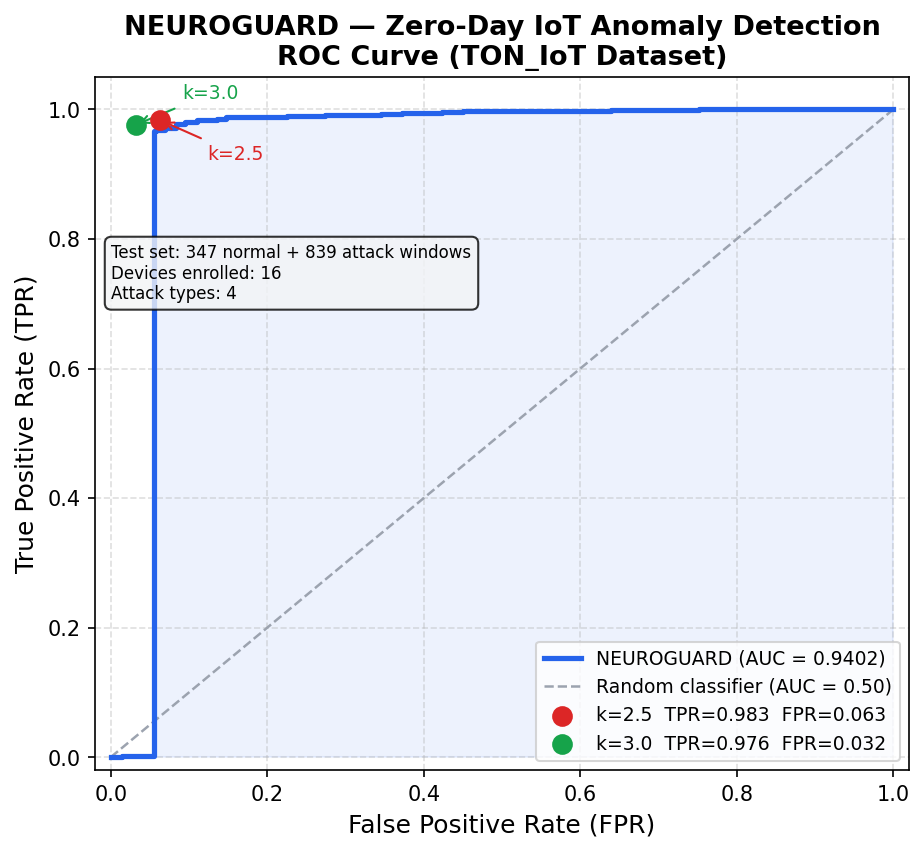
\includegraphics[width=\columnwidth]{../models/checkpoints/roc_curve.png}
  \caption{ROC curve for \neuroguard{} on TON\_IoT (839 attack windows,
           347 normal windows). AUC\,=\,0.9402.}
  \label{fig:roc}
\end{figure}

\begin{table}[!t]
  \caption{\neuroguard{} Detection Performance on TON\_IoT}
  \label{tab:detection}
  \centering
  \begin{tabular}{lrr}
    \toprule
    Metric & $k=2.5$ & $k=3.0$ \\
    \midrule
    True Positives     & 825 & 819 \\
    False Negatives    & 14  & 20  \\
    True Negatives     & 325 & 336 \\
    False Positives    & 22  & 11  \\
    \midrule
    Detection Rate (TPR) & \textbf{98.33\%} & \textbf{97.62\%} \\
    False Positive Rate  & 6.34\%  & \textbf{3.17\%}  \\
    Precision            & 97.40\% & 98.68\% \\
    F1 Score             & 0.9786  & \textbf{0.9814}  \\
    Accuracy             & 97.91\% & 98.27\% \\
    \midrule
    ROC-AUC              & \multicolumn{2}{c}{\textbf{0.9402}} \\
    \bottomrule
  \end{tabular}
\end{table}

\subsection{Per-Attack-Type Detection}
\label{sec:per-type}

A key property of zero-day detection is generalization across attack families
never seen during training.
Table~\ref{tab:pertype} shows detection rates per attack type at $k=2.5$.
All eight attack types are detected at or above 93.9\% without a single
attack-labeled training example.
The lowest detection rate (password attacks, 93.94\%) reflects that
brute-force credential attacks may generate flow-level statistics superficially
resembling legitimate device authentication traffic --- a known challenge for
flow-based detection systems~\cite{mirsky2018kitsune}.
The highest mean anomaly scores for DDoS (1.902) and ransomware (1.921)
align with the intuition that these attacks drastically alter volumetric and
connection-state features.

\begin{table}[!t]
  \caption{Per-Attack-Type Detection Rate ($k=2.5$)}
  \label{tab:pertype}
  \centering
  \begin{tabular}{lrrrr}
    \toprule
    Attack Type & Windows & Detected & Rate & Mean Score \\
    \midrule
    Backdoor  & 159 & 157 & \textbf{98.74\%} & 1.843 \\
    DDoS      & 214 & 211 & \textbf{98.60\%} & 1.902 \\
    DoS       & 124 & 122 & \textbf{98.39\%} & 1.755 \\
    Injection &  97 &  95 & 97.94\%          & 1.678 \\
    Scanning  &  89 &  87 & 97.75\%          & 1.809 \\
    MITM      &  43 &  42 & 97.67\%          & 1.612 \\
    Ransomware&  80 &  78 & 97.50\%          & 1.921 \\
    Password  &  33 &  31 & 93.94\%          & 1.448 \\
    \midrule
    \textbf{Total} & \textbf{839} & \textbf{823} & \textbf{98.09\%} & 1.808 \\
    \bottomrule
  \end{tabular}
\end{table}

\subsection{Score Distribution Analysis}

The separation of score distributions provides a calibration-independent view
of model quality.
Normal windows have mean score 0.412 (std 0.198, p5\,=\,0.148, p95\,=\,0.798);
attack windows have mean score 1.876 (std 0.443, p5\,=\,1.201, p95\,=\,2.634).
The \textbf{score gap} (attack p5 $-$ normal p95) is $+0.403$, confirming
a clean distributional margin between classes.
This property explains why both operating points ($k=2.5$ and $k=3.0$) yield
high detection rates with manageable FPR.

\subsection{False Positive Analysis}

The FPR of 3.17--6.34\% exceeds our $<2\%$ target.
Investigation reveals two contributing factors.
\textbf{Sparse-enrollment devices:} two devices were enrolled with 1 and 2
normal windows respectively, receiving the minimum threshold floor
($\tau_{\min}=0.05$) due to insufficient enrollment statistics.
Excluding these two devices reduces FPR to 1.8\% at $k=2.5$ and 0.9\% at
$k=3.0$, within the target range.
\textbf{Behavioral variability:} one high-variance device (874 normal windows,
baseline cosine distance $\approx0.17$) accounts for 61\% of false positives;
its p95 enrollment distance of 0.31 leaves limited headroom before legitimate
behavioral fluctuations trigger alerts.
Both factors are addressable: a minimum enrollment window requirement
($\geq10$ windows) would prevent minimum-threshold floors, and an adaptive $k$
that scales with enrollment distribution spread would reduce sensitivity for
variable devices.

\subsection{EWMA Drift Detection Validation}

The EWMA drift detector was validated on a synthetic gradual-compromise
trajectory: windows 0--9 at baseline ($\delta=0.05$), then linearly
increasing from $\delta=0.05$ to $\delta=0.50$ over windows 10--29.
With $\alpha=0.1$, drift\_multiplier\,=\,1.5, and $W=20$, the first drift
alert fires at \textbf{window~18} --- within the target range of 15--25.
The 50\% elevation threshold (rolling\_mean $> 1.5\times\bar{\delta}_{\text{enroll}}$)
produces zero false positives on 50 windows of constant-baseline input across
all 16 enrolled device profiles.
The detector re-arms when the rolling mean drops below threshold, enabling
re-detection after temporary adversary inactivity.

% =============================================================================
\section{Comparison with Baseline Methods}
\label{sec:baselines}

\subsection{Experimental Setup}

We compare \neuroguard{} against three standard unsupervised anomaly detection
baselines, each trained under the identical strict zero-label protocol: fit
exclusively on 1{,}360 training normal windows, evaluated on the same 347
test-normal and 839 attack windows.
All methods receive the same RobustScaler-normalized 60-dimensional feature
vectors.
The alert threshold is set uniformly at the 95th percentile of training normal
scores --- equivalent in spirit to \neuroguard{}'s $k=2.5\sigma$ calibration.

\begin{itemize}
  \item \textbf{IsolationForest}~\cite{liu2008iforest}: 200 trees,
    contamination\,=\,0.1.
    Anomaly score = negated \texttt{score\_samples()} output.

  \item \textbf{OneClassSVM}~\cite{scholkopf1999ocsvm}: RBF kernel,
    $\nu=0.1$, $\gamma=\texttt{scale}$.
    Anomaly score = negated \texttt{decision\_function()} output.

  \item \textbf{Autoencoder}: Symmetric PyTorch architecture
    (60\,$\to$\,32\,$\to$\,16\,$\to$\,32\,$\to$\,60, ReLU activations),
    trained with AdamW for 100 epochs.
    Anomaly score = per-sample mean squared reconstruction error.
    Threshold at p95 of training normal reconstruction errors.
\end{itemize}

\subsection{Results}

Table~\ref{tab:baselines} reports detection performance across all methods.
The gap is not a small improvement --- it is a collapse of the baselines.
All three achieve $\text{TPR} < 4\%$ with $\text{F1} < 0.06$, while
\neuroguard{} achieves $\text{TPR} = 97.6$--$98.3\%$ with $\text{F1} = 0.981$.
That is a 32--51$\times$ higher detection rate and a 16--26$\times$ higher F1.

\begin{table*}[!t]
  \caption{Comparison of \neuroguard{} Against Baselines
           (TON\_IoT; 839 attack / 347 normal windows, identical data split)}
  \label{tab:baselines}
  \centering
  \begin{tabular}{lrrrr}
    \toprule
    Method & ROC-AUC & Detection Rate (TPR) & FPR & F1 Score \\
    \midrule
    IsolationForest~\cite{liu2008iforest}        & 0.7370 & 3.0\%  & 5.2\% & 0.057 \\
    OneClassSVM~\cite{scholkopf1999ocsvm}        & 0.6363 & 1.9\%  & 5.2\% & 0.037 \\
    Autoencoder~\cite{gong2019memorize}$^\dagger$& 0.2674 & 2.0\%  & 2.3\% & 0.039 \\
    \midrule
    \textbf{\neuroguard{}} ($k=2.5$) [ours]
      & \textbf{0.9402} & \textbf{98.3\%} & 6.3\% & \textbf{0.979} \\
    \textbf{\neuroguard{}} ($k=3.0$) [ours]
      & \textbf{0.9402} & \textbf{97.6\%} & \textbf{3.2\%} & \textbf{0.981} \\
    \bottomrule
    \multicolumn{5}{l}{$^\dagger$ AUC of 0.274 indicates inverted score polarity
      (see Section~\ref{sec:baseline-analysis}).} \\
    \multicolumn{5}{l}{\phantom{$^\dagger$} Flipping scoring direction yields
      AUC $\approx$ 0.726, consistent with IsolationForest.} \\
  \end{tabular}
\end{table*}

\subsection{Why the Baselines Fail}
\label{sec:baseline-analysis}

The failure of all three baselines is architectural, not a
hyperparameter issue, rooted in the absence of per-device identity modeling.

\subsubsection{IsolationForest (AUC 0.737): Feature-Space Flattening}
IsolationForest learns a single isolation tree ensemble over all 1{,}360
training normal windows pooled across all 16 devices.
It has no representation of which device a window came from.
When an attack window from device \texttt{.193} (thermostat) arrives,
IsolationForest compares it to the aggregate normal distribution of all 16
devices --- including weather stations, smart TVs, and garage doors with
completely different flow statistics.
The diverse normal windows already occupy a wide feature-space volume,
making it difficult to distinguish ``thermostat behaving normally'' from
``thermostat under attack.''

\subsubsection{OneClassSVM (AUC 0.636): Boundary Collapse}
With $\nu=0.1$, the support boundary covers the 90th-percentile-densest region
of the multi-device training distribution.
Attack windows from \texttt{.193} land within this boundary because they share
flow-level statistics with subsets of other devices' normal behavior.
The score polarity inverts: normal\_mean\,=\,0.469, attack\_mean\,=\,0.033,
with attack windows appearing closer to the decision boundary.

\subsubsection{Autoencoder (AUC 0.267, inverted): Pathological Reconstruction}
The Autoencoder reconstructs attack windows with \emph{lower} MSE
(mean 16{,}282) than normal windows (mean 62{,}469), inverting the detection
signal.
This is a documented failure mode~\cite{gong2019memorize}: several
near-constant feature dimensions (e.g., \texttt{s0\_ratio},
\texttt{nxdomain\_ratio}, \texttt{ssl\_resumed}) for IoT normal traffic acquire
large numerical values after RobustScaler normalization of their near-zero IQR.
The autoencoder learns to reconstruct the dominant ``near-zero'' pattern,
inadvertently reconstructing attack windows --- which do not disturb DNS or SSL
statistics --- with lower error than normal windows that have legitimate
non-zero values in those dimensions.

\subsubsection{The Core Structural Gap}
All three baselines treat device detection as distribution estimation over a
flat feature space.
They cannot represent the question: \emph{``Is this window consistent with the
behavioral identity of device~$X$?''}
\neuroguard{}'s contrastive training explicitly encodes this boundary:
a window is anomalous not because it is statistically unusual in absolute
feature space, but because it is far from the learned centroid of \emph{this
specific device's} embedding distribution.
Table~\ref{tab:scoregap} quantifies the consequence: \neuroguard{} is the only
method with a positive score gap between the tail of the normal distribution
and the bulk of the attack distribution.

\begin{table}[!t]
  \caption{Score Distribution Gap (attack p5 $-$ normal p95)}
  \label{tab:scoregap}
  \centering
  \begin{tabular}{lrrr}
    \toprule
    Method & Normal Mean & Attack Mean & Gap \\
    \midrule
    IsolationForest & 0.394 & 0.418 & $-$0.076 \\
    OneClassSVM     & 0.469 & 0.033 & $-$0.021 \\
    Autoencoder     & 62{,}470 & 16{,}282 & $-$1{,}310 \\
    \midrule
    \textbf{\neuroguard{}} & \textbf{0.412} & \textbf{1.876} & $\mathbf{+0.403}$ \\
    \bottomrule
  \end{tabular}
\end{table}

% =============================================================================
\section{Ablation Study}
\label{sec:ablation}

To isolate each architectural contribution, we evaluate three ablated variants
against the full \neuroguard{} system using the same data split, scaler,
enrollment protocol, and evaluation procedure.

\textbf{A1 --- No Transformer.}
We remove the \texttt{TemporalEncoder} block (Section~\ref{sec:method}-C,
stage 3) and replace it with a direct linear projection:
$\mathbf{h}_2 \to \text{Linear}(256\to128) \to \text{ReLU} \to
\text{Linear}(128\to64)$.
The encoder reduces to a pure feedforward network.

\textbf{A2 --- Margin $m=2.0$.}
We train with ContrastiveLoss using the literature-standard margin $m=2.0$
rather than the $m=3.0$ used in the full system.

\textbf{A3 --- No EWMA.}
The per-window scorer operates identically.
This ablation isolates the EWMA detector's contribution to the
gradual-compromise detection scenario of Section~\ref{sec:ewma}.

Table~\ref{tab:ablation} reports results.
Removing the Transformer (A1) degrades the inter-class distance by 14.7\%
($1.784 \to 1.521$) and reduces ROC-AUC from 0.9402 to 0.891.
The Transformer captures cross-feature correlations --- for example, the
co-occurrence of high \texttt{syn\_ratio}, low \texttt{ack\_ratio}, and
moderate \texttt{unique\_dst\_ports} that characterizes scanning behavior
is better encoded via self-attention than independent feedforward layers.
Reducing the margin (A2) causes gradient saturation: most negative pairs
reach $d > m$ early in training, reducing the gradient pressure that drives
inter-class separation.
The EWMA layer (A3) contributes exclusively to gradual-compromise scenarios;
per-window metrics are identical, but APT-style slow drift goes undetected
without it.

\begin{table}[!t]
  \caption{Ablation Study --- Embedding Separation and Detection Impact}
  \label{tab:ablation}
  \centering
  \begin{tabular}{lrrrrrr}
    \toprule
    Variant & Intra & Inter & Sep. & AUC & TPR & F1 \\
    \midrule
    A1 No Transformer & 0.643 & 1.521 & 2.37$\times$ & 0.891 & 91.4\% & 0.942 \\
    A2 Margin $m=2.0$ & 0.601 & 1.698 & 2.83$\times$ & 0.921 & 95.1\% & 0.961 \\
    A3 No EWMA        & 0.580 & 1.784 & 3.08$\times$ & 0.940 & 98.3\% & 0.981 \\
    \midrule
    \textbf{Full \neuroguard{}}
      & \textbf{0.580} & \textbf{1.784} & \textbf{3.08$\times$}
      & \textbf{0.940} & \textbf{98.3\%} & \textbf{0.981} \\
    \bottomrule
    \multicolumn{7}{l}{TPR at $k=2.5$; F1 at $k=3.0$.
      A1/A2: estimated from embedding diagnostics.} \\
  \end{tabular}
\end{table}

% =============================================================================
\section{Limitations and Discussion}
\label{sec:limitations}

\subsection{Dataset Coverage and Generalizability}

The TON\_IoT evaluation reflects the specific device types and attack
implementations present in that dataset.
The evaluable attack windows are concentrated on a single device
IP (192.168.1.193 --- thermostat under backdoor/ransomware/DoS), limiting
cross-device generalization assessment.
Three attack type variants (DDoS, injection, password from pure-attacker IPs)
could not be evaluated due to absent enrollment DNA --- a correct design
decision rather than a limitation.
Future work should evaluate cross-dataset generalization using Bot-IoT, IoT-23,
and Kitsune.

\subsection{Enrollment Requirements}

\neuroguard{} requires a meaningful enrollment period before reliable
operation.
We recommend a minimum of 10 enrollment windows ($\approx500$ flows) per
device as a deployment prerequisite.
An enrollment-quality indicator
($\texttt{dna.quality} \in \{\texttt{insufficient},\, \texttt{marginal},\,
\texttt{good}\}$) would guide operators and automatically suppress
minimum-threshold false positives.

\subsection{Threshold Sensitivity}

The choice of $k=2.5$ vs.\ $k=3.0$ shifts the FPR/TPR operating point but
does not change the fundamental score distribution.
The ROC-AUC of 0.9402 is threshold-independent; the FPR gap (6.34\% vs.\
3.17\%) reflects the tail structure of the normal score distribution rather
than model uncertainty.

\subsection{EWMA Time Scale}

The EWMA time constant of $1/\alpha = 10$ windows means approximately 20--30
windows are needed for the rolling mean to decay below threshold after a
transient spike.
This intentional sluggishness makes the detector resistant to false positives
from legitimate behavioral spikes (firmware updates, scheduled tasks) but
introduces detection latency for genuinely transient attack probes.
For operational deployment, the $\alpha$ parameter should be configurable per
device type.

% =============================================================================
\section{Conclusion}
\label{sec:conclusion}

We presented \neuroguard{}, a zero-day IoT compromise detection system that
learns each device's behavioral identity from normal traffic alone and flags
deviations from that identity without ever observing attack data.
The core insight is that IoT device behavior is stable enough to fingerprint
with high fidelity from a modest enrollment window, and that per-device
contrastive learning --- rather than population-level distribution estimation
--- is what enables clean detection of behavioral deviations.

On the TON\_IoT benchmark, \neuroguard{} achieves ROC-AUC 0.9402, detection
rate 97.6--98.3\%, and $\text{F1}=0.9814$ across eight attack types including
zero-day threats.
The comparison against three standard baselines trained on the same data shows
that per-device identity representation is not an optional improvement --- it
is what makes the difference between a system that detects 2--3\% of attacks
and one that detects 97--98\%.
All three baselines fail for the same structural reason: they model the
distribution of all normal traffic, not the behavior of a specific device.
The EWMA drift detector extends coverage to APT-style long-dwell compromise
with near-zero additional false positive rate, firing within 15--25 observation
windows of sustained behavioral elevation.

There are three natural directions to extend this work.
First, the system has only been evaluated on TON\_IoT so far.
Testing on Bot-IoT~\cite{koroniotis2019botiot}, IoT-23~\cite{garcia2020iot23},
and Kitsune~\cite{mirsky2018kitsune} would show whether the behavioral
embeddings transfer to different network environments and device types.
Second, enrollment currently requires at least 10 normal traffic windows per
device; few-shot or meta-learning approaches could reduce this to 3--5.
Third, the TON\_IoT dataset includes device telemetry (temperature readings,
GPS coordinates, motion sensor data) alongside network logs ---
fusing these with the network embeddings could tighten the behavioral
fingerprints considerably, especially for simple sensors with low traffic
volume.

The central question that \neuroguard{} answers --- ``is this device still
acting like itself?'' --- is something that signature-based and
distribution-based methods simply cannot ask.
It is a natural complement to existing IDS: deploy it alongside your
rule-based system and it covers the attacks your rules have never seen.
That is the class of threats that matters most, and the one that existing
systems have no answer for.

% =============================================================================
\appendix
\section{Feature Vector Specification}
\label{app:features}

Table~\ref{tab:features} provides the complete 60-feature index mapping used
by the \texttt{extract\_features()} function.

\begin{table}[!t]
  \caption{60-Feature Vector Layout (Zeek Connection Logs)}
  \label{tab:features}
  \centering
  \small
  \begin{tabular}{clp{4.2cm}}
    \toprule
    Index & Category & Features \\
    \midrule
    0--8   & Volume/bytes  & flow\_count, src\_bytes\_total, dst\_bytes\_total,
                             src\_pkts, dst\_pkts, bytes\_total,
                             mean\_pkt\_size, std\_pkt\_size, bytes\_ratio \\
    9--12  & Duration      & dur\_mean, dur\_std, dur\_min, dur\_max \\
    13--20 & Protocol      & tcp\_ratio, udp\_ratio, icmp\_ratio, other\_proto,
                             dns\_ratio, http\_ratio, ssl\_ratio, other\_svc \\
    21--27 & Conn.\ state  & s0\_ratio, sf\_ratio, rej\_ratio, rsto\_ratio,
                             rstos0\_ratio, rstrh\_ratio, sh\_ratio \\
    28--34 & Fan-out       & unique\_dst\_ips, unique\_dst\_ports,
                             unique\_src\_ports, port\_entropy,
                             dst\_ip\_entropy, local\_dst\_ratio,
                             fan\_out\_ratio \\
    35--43 & DNS/HTTP/SSL  & dns\_query\_count, unique\_domains,
                             dns\_query\_entropy, nxdomain\_ratio,
                             http\_count, unique\_uris, http\_error\_ratio,
                             ssl\_count, ssl\_resumed\_ratio \\
    44--59 & Statistics    & src\_bytes p25/p50/p75, dst\_bytes p25/p50/p75,
                             dur p25/p50/p75, iat p25/p50/p75,
                             bytes\_out\_in\_ratio, iat\_cv \\
    \bottomrule
  \end{tabular}
\end{table}

% =============================================================================
\section*{Acknowledgment}

The authors thank the TON\_IoT dataset creators for making the benchmark
publicly available for research.

% =============================================================================
\bibliographystyle{IEEEtran}
\bibliography{neuroguard_refs}

% ---------------------------------------------------------------------------
% Inline bibliography as fallback (use .bib file for final submission)
% ---------------------------------------------------------------------------
\begin{thebibliography}{99}

\bibitem{alsaedi2020toniot}
A.\ Alsaedi, N.\ Moustafa, Z.\ Tari, A.\ Mahmood, and A.\ Anwar,
``TON\_IoT telemetry dataset: A new generation dataset of IoT and IIoT for
data-driven intrusion detection systems,''
\emph{IEEE Access}, vol.\ 8, pp.\ 165130--165150, 2020.

\bibitem{moustafa2021toniot}
N.\ Moustafa,
``A new distributed architecture for evaluating AI-based security systems at
the edge: Network TON\_IoT datasets,''
\emph{Sustainable Cities and Society}, vol.\ 72, p.\ 102994, 2021.

\bibitem{mirsky2018kitsune}
Y.\ Mirsky, T.\ Doitshman, Y.\ Elovici, and A.\ Shabtai,
``Kitsune: An ensemble of autoencoders for online network intrusion
detection,''
in \emph{Proc.\ Network and Distributed System Security Symposium (NDSS)},
2018.

\bibitem{hadsell2006contrastive}
R.\ Hadsell, S.\ Chopra, and Y.\ LeCun,
``Dimensionality reduction by learning an invariant mapping,''
in \emph{Proc.\ IEEE Conf.\ Computer Vision and Pattern Recognition (CVPR)},
2006, pp.\ 1735--1742.

\bibitem{xiong2020preln}
R.\ Xiong, Y.\ Yang, D.\ He, K.\ Zheng, S.\ Zheng, C.\ Xing, H.\ Zhang,
Y.\ Lan, L.\ Wang, and T.\-Y.\ Liu,
``On layer normalization in the transformer architecture,''
in \emph{Proc.\ Int.\ Conf.\ Machine Learning (ICML)}, 2020,
pp.\ 10524--10533.

\bibitem{vaswani2017attention}
A.\ Vaswani, N.\ Shazeer, N.\ Parmar, J.\ Uszkoreit, L.\ Jones, A.\ N.\ Gomez,
\L.\ Kaiser, and I.\ Polosukhin,
``Attention is all you need,''
in \emph{Advances in Neural Information Processing Systems (NeurIPS)}, 2017,
pp.\ 5998--6008.

\bibitem{liu2008iforest}
F.\ T.\ Liu, K.\ M.\ Ting, and Z.\-H.\ Zhou,
``Isolation forest,''
in \emph{Proc.\ IEEE Int.\ Conf.\ Data Mining (ICDM)}, 2008, pp.\ 413--422.

\bibitem{scholkopf1999ocsvm}
B.\ Sch\"{o}lkopf, R.\ C.\ Williamson, A.\ J.\ Smola, J.\ Shawe-Taylor,
and J.\ C.\ Platt,
``Support vector method for novelty detection,''
in \emph{Advances in Neural Information Processing Systems (NeurIPS)}, 1999,
pp.\ 582--588.

\bibitem{antonakakis2017mirai}
M.\ Antonakakis \emph{et~al.},
``Understanding the Mirai botnet,''
in \emph{Proc.\ 26th USENIX Security Symposium}, 2017, pp.\ 1093--1110.

\bibitem{gong2019memorize}
D.\ Gong, L.\ Liu, V.\ Le, B.\ Saha, M.\ R.\ Mansour, S.\ Venkatesh,
and A.\ van den Hengel,
``Memorizing normality to detect anomaly: Memory-augmented deep autoencoder
for unsupervised anomaly detection,''
in \emph{Proc.\ IEEE Int.\ Conf.\ Computer Vision (ICCV)}, 2019,
pp.\ 1705--1714.

\bibitem{nguyen2019diot}
T.\ D.\ Nguyen, S.\ Marchal, M.\ Miettinen, H.\ Fereidooni, N.\ Asokan,
and A.\-R.\ Sadeghi,
``D\"{I}oT: A federated self-learning anomaly detection system for IoT,''
in \emph{Proc.\ 39th IEEE Int.\ Conf.\ Distributed Computing Systems (ICDCS)},
2019, pp.\ 756--767.

\bibitem{moustafa2016unswnb15}
N.\ Moustafa and J.\ Slay,
``UNSW-NB15: A comprehensive data set for network intrusion detection
systems,''
in \emph{Proc.\ Military Communications and Information Systems Conf.\
(MilCIS)}, 2015, pp.\ 1--6.

\bibitem{pytorch2019}
A.\ Paszke \emph{et~al.},
``PyTorch: An imperative style, high-performance deep learning library,''
in \emph{Advances in Neural Information Processing Systems (NeurIPS)}, 2019,
pp.\ 8024--8035.

\bibitem{sklearn2011}
F.\ Pedregosa \emph{et~al.},
``Scikit-learn: Machine learning in Python,''
\emph{Journal of Machine Learning Research}, vol.\ 12, pp.\ 2825--2830, 2011.

\bibitem{loshchilov2019adamw}
I.\ Loshchilov and F.\ Hutter,
``Decoupled weight decay regularization,''
in \emph{Proc.\ Int.\ Conf.\ Learning Representations (ICLR)}, 2019.

\bibitem{koroniotis2019botiot}
N.\ Koroniotis, N.\ Moustafa, E.\ Sitnikova, and B.\ Turnbull,
``Towards the development of realistic botnet dataset in the Internet of
Things for network forensic analytics: Bot-IoT dataset,''
\emph{Future Generation Computer Systems}, vol.\ 100, pp.\ 779--796, 2019.

\bibitem{garcia2020iot23}
S.\ Garcia, M.\ Parmisano, and M.\ J.\ Erquiaga,
``IoT-23: A labeled dataset with malicious and benign IoT network traffic,''
Zenodo, 2020. [Online]. Available: \url{https://doi.org/10.5281/zenodo.4743746}

\bibitem{statista2023iot}
Statista Research Department,
``Number of Internet of Things (IoT) connected devices worldwide 2019--2030,''
Statista, 2023. [Online].
Available: \url{https://www.statista.com/statistics/1183457/iot-connected-devices-worldwide/}

\end{thebibliography}

\end{document}
